\documentclass[10pt,conference]{IEEEtran}
\IEEEoverridecommandlockouts
\usepackage[T1]{fontenc}
\usepackage{cite}
\usepackage{amsmath,amssymb}
\usepackage{graphicx}
\usepackage{booktabs}
\usepackage{xcolor}
\usepackage{url}
\usepackage{xspace}
\usepackage{pgfplots}
% Shipped with compat=1.18 (current pgfplots). This machine's TeX Live 2020 has pgfplots 1.17, so
% `make pdf` in artifact/ builds a copy with compat=1.17; the source here stays at 1.18.
\pgfplotsset{compat=1.18}
\usepgfplotslibrary{fillbetween}
\usetikzlibrary{arrows.meta}
\usepackage[hidelinks]{hyperref}

% generated by artifact/src/render.py -- do not edit
\newcommand{\XAExtractionCountRho}{0.42}
\newcommand{\XAExtractionN}{30}
\newcommand{\XAFrameNeg}{619}
\newcommand{\XAFramePos}{155}
\newcommand{\XAJudgeAnchorAgreePct}{62.3}
\newcommand{\XAJudgeAnchorDeadBulk}{2.5}
\newcommand{\XAJudgeAnchorDeadSecond}{7.0}
\newcommand{\XAJudgeAnchorKappa}{0.16}
\newcommand{\XAJudgeAnchorKappaDead}{0.35}
\newcommand{\XAJudgeAnchorKappaDeadUnweighted}{0.35}
\newcommand{\XAJudgeAnchorN}{284}
\newcommand{\XAJudgeAnchorPairs}{21}
\newcommand{\XAJudgeAnchorPrecision}{71.4}
\newcommand{\XAJudgeAnchorRecall}{25.0}
\newcommand{\XAJudgeAnchorSecondConWhereBulkNot}{5.4}
\newcommand{\XAJudgeCommitAgreePct}{65.9}
\newcommand{\XAJudgeCommitDeadBulk}{2.4}
\newcommand{\XAJudgeCommitDeadSecond}{7.8}
\newcommand{\XAJudgeCommitKappa}{0.09}
\newcommand{\XAJudgeCommitKappaDead}{0.21}
\newcommand{\XAJudgeCommitKappaDeadUnweighted}{0.36}
\newcommand{\XAJudgeCommitN}{864}
\newcommand{\XAJudgeCommitPairs}{75}
\newcommand{\XAJudgeCommitPrecision}{51.9}
\newcommand{\XAJudgeCommitRecall}{15.7}
\newcommand{\XAJudgeCommitSecondConWhereBulkNot}{6.7}
\newcommand{\XAJudgePairsTotal}{125}
\newcommand{\XAJudgePairsValid}{96}
\newcommand{\XATypeKappa}{0.62}
\newcommand{\XATypeNClaims}{460}
\newcommand{\XAdjudicatedN}{2}
\newcommand{\XAnchorContradictedNDoc}{43}
\newcommand{\XAnchorContradictedNLlm}{19}
\newcommand{\XAnchorContradictedPctDoc}{13.9}
\newcommand{\XAnchorContradictedPctDocAudited}{1.6}
\newcommand{\XAnchorContradictedPctLlm}{1.3}
\newcommand{\XAnchorDate}{2024-11-01}
\newcommand{\XAnchorUnresolvedPctDoc}{11.0}
\newcommand{\XAnchorUnresolvedPctLlm}{3.0}
\newcommand{\XAtomicBehaviouralDeadK}{10.7}
\newcommand{\XAtomicDataflowDeadK}{15.4}
\newcommand{\XAtomicIntentDeadK}{7.3}
\newcommand{\XAtomicStructuralDeadK}{13.5}
\newcommand{\XAuditAmbiguous}{3}
\newcommand{\XAuditDecomposerError}{18}
\newcommand{\XAuditJudgeError}{17}
\newcommand{\XAuditRealStale}{5}
\newcommand{\XBulkModel}{qwen2.5-coder:14b}
\newcommand{\XCTCallChangeHR}{2.90}
\newcommand{\XCTCallChangeHRHi}{4.23}
\newcommand{\XCTCallChangeHRLo}{1.99}
\newcommand{\XCTCallChangeN}{460}
\newcommand{\XCTCallChangeRate}{4.3}
\newcommand{\XCTCallReceiverHR}{1.81}
\newcommand{\XCTCallReceiverHRHi}{3.43}
\newcommand{\XCTCallReceiverHRLo}{0.96}
\newcommand{\XCTCallReceiverN}{41}
\newcommand{\XCTCallReceiverRate}{2.0}
\newcommand{\XCTControlFlowHR}{0.85}
\newcommand{\XCTControlFlowHRHi}{1.19}
\newcommand{\XCTControlFlowHRLo}{0.61}
\newcommand{\XCTControlFlowN}{329}
\newcommand{\XCTControlFlowRate}{4.1}
\newcommand{\XCTExceptionHR}{1.44}
\newcommand{\XCTExceptionHRHi}{2.18}
\newcommand{\XCTExceptionHRLo}{0.95}
\newcommand{\XCTExceptionN}{85}
\newcommand{\XCTExceptionRate}{6.2}
\newcommand{\XCTIdentifierRenameHR}{1.53}
\newcommand{\XCTIdentifierRenameHRHi}{3.58}
\newcommand{\XCTIdentifierRenameHRLo}{0.65}
\newcommand{\XCTIdentifierRenameN}{59}
\newcommand{\XCTIdentifierRenameRate}{1.3}
\newcommand{\XCTLiteralOrKeywordN}{27}
\newcommand{\XCTLiteralOrKeywordRate}{0.4}
\newcommand{\XCTLocalEditN}{294}
\newcommand{\XCTLocalEditRate}{0.8}
\newcommand{\XCTReturnValueHR}{1.58}
\newcommand{\XCTReturnValueHRHi}{3.11}
\newcommand{\XCTReturnValueHRLo}{0.80}
\newcommand{\XCTReturnValueN}{27}
\newcommand{\XCTReturnValueRate}{5.9}
\newcommand{\XCTSignatureHR}{2.44}
\newcommand{\XCTSignatureHRHi}{3.49}
\newcommand{\XCTSignatureHRLo}{1.70}
\newcommand{\XCTSignatureN}{114}
\newcommand{\XCTSignatureRate}{6.8}
\newcommand{\XClaimsPerDoc}{4.8}
\newcommand{\XClaimsPerExpl}{11.1}
\newcommand{\XCloglogClusters}{128}
\newcommand{\XCloglogCompoundCompound}{2.09}
\newcommand{\XCloglogCompoundCompoundHi}{2.81}
\newcommand{\XCloglogCompoundCompoundLo}{1.55}
\newcommand{\XCloglogCompoundTyBehavioural}{0.72}
\newcommand{\XCloglogCompoundTyBehaviouralHi}{1.04}
\newcommand{\XCloglogCompoundTyBehaviouralLo}{0.50}
\newcommand{\XCloglogCompoundTyIntent}{0.34}
\newcommand{\XCloglogCompoundTyIntentHi}{0.84}
\newcommand{\XCloglogCompoundTyIntentLo}{0.13}
\newcommand{\XCloglogCompoundTyStructural}{0.89}
\newcommand{\XCloglogCompoundTyStructuralHi}{1.15}
\newcommand{\XCloglogCompoundTyStructuralLo}{0.68}
\newcommand{\XCloglogCtCallChange}{2.90}
\newcommand{\XCloglogCtCallChangeHi}{4.23}
\newcommand{\XCloglogCtCallChangeLo}{1.99}
\newcommand{\XCloglogCtCallReceiver}{1.81}
\newcommand{\XCloglogCtCallReceiverHi}{3.43}
\newcommand{\XCloglogCtCallReceiverLo}{0.96}
\newcommand{\XCloglogCtControlFlow}{0.85}
\newcommand{\XCloglogCtControlFlowHi}{1.19}
\newcommand{\XCloglogCtControlFlowLo}{0.61}
\newcommand{\XCloglogCtException}{1.44}
\newcommand{\XCloglogCtExceptionHi}{2.18}
\newcommand{\XCloglogCtExceptionLo}{0.95}
\newcommand{\XCloglogCtIdentifierRename}{1.53}
\newcommand{\XCloglogCtIdentifierRenameHi}{3.58}
\newcommand{\XCloglogCtIdentifierRenameLo}{0.65}
\newcommand{\XCloglogCtReturnValue}{1.58}
\newcommand{\XCloglogCtReturnValueHi}{3.11}
\newcommand{\XCloglogCtReturnValueLo}{0.80}
\newcommand{\XCloglogCtSignature}{2.44}
\newcommand{\XCloglogCtSignatureHi}{3.49}
\newcommand{\XCloglogCtSignatureLo}{1.70}
\newcommand{\XCloglogEvents}{250}
\newcommand{\XCloglogLogLinesFile}{1.39}
\newcommand{\XCloglogLogLinesFileHi}{1.61}
\newcommand{\XCloglogLogLinesFileLo}{1.20}
\newcommand{\XCloglogLogLinesFn}{1.35}
\newcommand{\XCloglogLogLinesFnHi}{1.62}
\newcommand{\XCloglogLogLinesFnLo}{1.13}
\newcommand{\XCloglogPeriods}{9772}
\newcommand{\XCloglogTyBehavioural}{0.73}
\newcommand{\XCloglogTyBehaviouralHi}{1.05}
\newcommand{\XCloglogTyBehaviouralLo}{0.51}
\newcommand{\XCloglogTyIntent}{0.32}
\newcommand{\XCloglogTyIntentHi}{0.79}
\newcommand{\XCloglogTyIntentLo}{0.13}
\newcommand{\XCloglogTyStructural}{1.06}
\newcommand{\XCloglogTyStructuralHi}{1.38}
\newcommand{\XCloglogTyStructuralLo}{0.81}
\newcommand{\XCloglogUnadjTyBehavioural}{0.66}
\newcommand{\XCloglogUnadjTyBehaviouralHi}{0.96}
\newcommand{\XCloglogUnadjTyBehaviouralLo}{0.46}
\newcommand{\XCloglogUnadjTyIntent}{0.32}
\newcommand{\XCloglogUnadjTyIntentHi}{0.81}
\newcommand{\XCloglogUnadjTyIntentLo}{0.13}
\newcommand{\XCloglogUnadjTyStructural}{1.05}
\newcommand{\XCloglogUnadjTyStructuralHi}{1.38}
\newcommand{\XCloglogUnadjTyStructuralLo}{0.80}
\newcommand{\XCohortNDoc}{233}
\newcommand{\XCohortNLlm}{1354}
\newcommand{\XCompoundPctLlm}{15.8}
\newcommand{\XCoxUnpenCtCallChange}{2.89}
\newcommand{\XCoxUnpenCtCallChangeHi}{4.44}
\newcommand{\XCoxUnpenCtCallChangeLo}{1.89}
\newcommand{\XCoxUnpenCtCallReceiver}{1.81}
\newcommand{\XCoxUnpenCtCallReceiverHi}{3.63}
\newcommand{\XCoxUnpenCtCallReceiverLo}{0.90}
\newcommand{\XCoxUnpenCtControlFlow}{0.86}
\newcommand{\XCoxUnpenCtControlFlowHi}{1.32}
\newcommand{\XCoxUnpenCtControlFlowLo}{0.56}
\newcommand{\XCoxUnpenCtException}{1.44}
\newcommand{\XCoxUnpenCtExceptionHi}{2.86}
\newcommand{\XCoxUnpenCtExceptionLo}{0.72}
\newcommand{\XCoxUnpenCtIdentifierRename}{1.52}
\newcommand{\XCoxUnpenCtIdentifierRenameHi}{3.96}
\newcommand{\XCoxUnpenCtIdentifierRenameLo}{0.58}
\newcommand{\XCoxUnpenCtReturnValue}{1.65}
\newcommand{\XCoxUnpenCtReturnValueHi}{4.32}
\newcommand{\XCoxUnpenCtReturnValueLo}{0.63}
\newcommand{\XCoxUnpenCtSignature}{2.41}
\newcommand{\XCoxUnpenCtSignatureHi}{4.19}
\newcommand{\XCoxUnpenCtSignatureLo}{1.39}
\newcommand{\XCoxUnpenLogLinesFile}{1.39}
\newcommand{\XCoxUnpenLogLinesFileHi}{1.64}
\newcommand{\XCoxUnpenLogLinesFileLo}{1.18}
\newcommand{\XCoxUnpenLogLinesFn}{1.35}
\newcommand{\XCoxUnpenLogLinesFnHi}{1.74}
\newcommand{\XCoxUnpenLogLinesFnLo}{1.05}
\newcommand{\XCoxUnpenOk}{True}
\newcommand{\XCoxUnpenTyBehavioural}{0.74}
\newcommand{\XCoxUnpenTyBehaviouralHi}{1.13}
\newcommand{\XCoxUnpenTyBehaviouralLo}{0.48}
\newcommand{\XCoxUnpenTyIntent}{0.32}
\newcommand{\XCoxUnpenTyIntentHi}{0.84}
\newcommand{\XCoxUnpenTyIntentLo}{0.12}
\newcommand{\XCoxUnpenTyStructural}{1.06}
\newcommand{\XCoxUnpenTyStructuralHi}{1.40}
\newcommand{\XCoxUnpenTyStructuralLo}{0.80}
\newcommand{\XDeadPctKMain}{15.4}
\newcommand{\XDeadRepoAiohttp}{12.0}
\newcommand{\XDeadRepoAttrs}{0.0}
\newcommand{\XDeadRepoBlack}{10.1}
\newcommand{\XDeadRepoClick}{41.5}
\newcommand{\XDeadRepoHypothesis}{18.8}
\newcommand{\XDeadRepoPip}{14.5}
\newcommand{\XDeadRepoPydantic}{15.5}
\newcommand{\XDeadRepoPylint}{3.3}
\newcommand{\XDeadRepoPytest}{24.2}
\newcommand{\XDeadRepoSphinx}{10.3}
\newcommand{\XDeadRepoTextual}{15.3}
\newcommand{\XDisagreementN}{170}
\newcommand{\XDocAuditCoverage}{43/43}
\newcommand{\XDocAuditDecomposerMaxFunc}{11}
\newcommand{\XDocAuditN}{43}
\newcommand{\XDocAuditRealPct}{11.6}
\newcommand{\XDuplicateQualnameExcluded}{250}
\newcommand{\XEligiblePopulation}{12926}
\newcommand{\XEligiblePopulationClean}{10903}
\newcommand{\XFollowK}{6}
\newcommand{\XFormatOnlyLooks}{228}
\newcommand{\XFreshCrossKappa}{0.72}
\newcommand{\XFreshCrossN}{60}
\newcommand{\XFreshDocN}{65}
\newcommand{\XFreshRawAgree}{55}
\newcommand{\XFreshRedrawN}{80}
\newcommand{\XFreshResN}{232}
\newcommand{\XFreshResSupported}{121}
\newcommand{\XFreshResUnparsed}{33}
\newcommand{\XFreshWeightedAgree}{97.3}
\newcommand{\XHFourAgeMedianDoc}{3.0}
\newcommand{\XHFourAgeNDocClaims}{178}
\newcommand{\XHFourAgeNDocFunctions}{43}
\newcommand{\XHFourAgeNLlmClaimsRestricted}{445}
\newcommand{\XHFourDeadPctDoc}{4.8}
\newcommand{\XHFourDeadPctLlm}{16.4}
\newcommand{\XHFourDeathsDoc}{11}
\newcommand{\XHFourDeathsLlm}{106}
\newcommand{\XHFourDocDeathFunctions}{10}
\newcommand{\XHFourFalseAtKDoc}{17.0}
\newcommand{\XHFourFalseAtKLlm}{17.3}
\newcommand{\XHFourFunctionsDocWorse}{6}
\newcommand{\XHFourFunctionsLlmWorse}{41}
\newcommand{\XHFourNDocClaims}{227}
\newcommand{\XHFourNFunctions}{62}
\newcommand{\XHFourNLlmClaims}{647}
\newcommand{\XHFourP}{{\le}0.001}
\newcommand{\XHFourPHolm}{{\le}0.001}
\newcommand{\XHFourPHolmMFour}{{\le}0.001}
\newcommand{\XHFourPRaw}{{\le}0.001}
\newcommand{\XHFourPairedDiffHi}{17.2}
\newcommand{\XHFourPairedDiffLo}{8.8}
\newcommand{\XHFourPairedDiffPct}{12.9}
\newcommand{\XHFourVerdict}{inconclusive}
\newcommand{\XHFourYoungDeadDoc}{5.3}
\newcommand{\XHFourYoungDeadLlm}{16.0}
\newcommand{\XHFourYoungDeathsDoc}{8}
\newcommand{\XHFourYoungNFunctions}{31}
\newcommand{\XHHr}{3.47}
\newcommand{\XHHrDelayed}{2.87}
\newcommand{\XHHrDelayedHi}{17.47}
\newcommand{\XHHrDelayedLo}{0.47}
\newcommand{\XHHrDelayedStrat}{2.92}
\newcommand{\XHHrDelayedStratHi}{11.13}
\newcommand{\XHHrDelayedStratLo}{0.76}
\newcommand{\XHHrHi}{6.22}
\newcommand{\XHHrLo}{1.94}
\newcommand{\XHOneAucFn}{0.68}
\newcommand{\XHOneAucFnHi}{0.73}
\newcommand{\XHOneAucFnLo}{0.64}
\newcommand{\XHOneMcse}{0.003}
\newcommand{\XHOneNPairs}{1014}
\newcommand{\XHOnePHolm}{{=}0.068}
\newcommand{\XHOnePHolmMFour}{{=}0.137}
\newcommand{\XHOnePRaw}{{=}0.068}
\newcommand{\XHOnePSeedMax}{{=}0.086}
\newcommand{\XHOnePSeedMin}{{=}0.053}
\newcommand{\XHOnePWeak}{{=}0.068}
\newcommand{\XHOnePWeakMcse}{{=}0.003}
\newcommand{\XHOnePairsWithDeathPct}{17.5}
\newcommand{\XHOneRhoFile}{0.24}
\newcommand{\XHOneRhoFileHi}{0.30}
\newcommand{\XHOneRhoFileLo}{0.18}
\newcommand{\XHOneRhoFn}{0.25}
\newcommand{\XHOneRhoFnHi}{0.31}
\newcommand{\XHOneRhoFnLo}{0.19}
\newcommand{\XHOneSeedMax}{0.086}
\newcommand{\XHOneSeedMin}{0.053}
\newcommand{\XHOneSeedsGeZeroFivePct}{100.0}
\newcommand{\XHOneVerdict}{inconclusive}
\newcommand{\XHOneVerdictMFour}{inconclusive}
\newcommand{\XHOneZeroShare}{82.5}
\newcommand{\XHThreeDegenerate}{True}
\newcommand{\XHThreeIdentFa}{1.4}
\newcommand{\XHThreeIdentFaHi}{3.5}
\newcommand{\XHThreeIdentFaLo}{0.0}
\newcommand{\XHThreeIdentFaStrict}{0.0}
\newcommand{\XHThreeIdentRecall}{51.7}
\newcommand{\XHThreeIdentRecallHi}{62.4}
\newcommand{\XHThreeIdentRecallLo}{39.3}
\newcommand{\XHThreeKZeroN}{129}
\newcommand{\XHThreeKZeroVThreeMean}{1.2}
\newcommand{\XHThreeKZeroVTwoFlag}{100.0}
\newcommand{\XHThreeNAsked}{363}
\newcommand{\XHThreeNDeadClaims}{205}
\newcommand{\XHThreeNNeg}{141}
\newcommand{\XHThreeNNegAnchorWrong}{59}
\newcommand{\XHThreeNNegStrict}{82}
\newcommand{\XHThreeNPos}{147}
\newcommand{\XHThreeVOneFa}{100.0}
\newcommand{\XHThreeVOneFaStrict}{100.0}
\newcommand{\XHThreeVOneRecall}{100.0}
\newcommand{\XHThreeVThreeAuc}{0.58}
\newcommand{\XHThreeVThreeAucHi}{0.61}
\newcommand{\XHThreeVThreeAucLo}{0.55}
\newcommand{\XHThreeVThreeAucVsKZero}{0.74}
\newcommand{\XHThreeVThreeMeanNeg}{1.9}
\newcommand{\XHThreeVThreeMeanPos}{2.4}
\newcommand{\XHThreeVThreeParsedPct}{100.0}
\newcommand{\XHThreeVTwoFa}{100.0}
\newcommand{\XHThreeVTwoFaStrict}{100.0}
\newcommand{\XHThreeVTwoRecall}{100.0}
\newcommand{\XHThreeVerdict}{inconclusive}
\newcommand{\XHTwoBehaviouralHighest}{False}
\newcommand{\XHTwoBootB}{2000}
\newcommand{\XHTwoBootMax}{0.033}
\newcommand{\XHTwoBootMcse}{0.004}
\newcommand{\XHTwoBootMin}{0.025}
\newcommand{\XHTwoBootPMcse}{{=}0.004}
\newcommand{\XHTwoBootPSeedMax}{{=}0.033}
\newcommand{\XHTwoBootPSeedMin}{{=}0.025}
\newcommand{\XHTwoBootSkipDiverged}{105}
\newcommand{\XHTwoBootSkipNoIntent}{12}
\newcommand{\XHTwoBootSkipPeriod}{178}
\newcommand{\XHTwoBootSkipped}{295}
\newcommand{\XHTwoIntentDeathFunctions}{5}
\newcommand{\XHTwoIntentDeaths}{6}
\newcommand{\XHTwoIntentDeathsClick}{4}
\newcommand{\XHTwoIntentLowest}{True}
\newcommand{\XHTwoPHolm}{{=}0.032}
\newcommand{\XHTwoPHolmMFour}{{=}0.048}
\newcommand{\XHTwoPRaw}{{=}0.016}
\newcommand{\XHTwoVerdict}{type effect, predicted ordering not supported}
\newcommand{\XHTwoWaldBootP}{{=}0.033}
\newcommand{\XHTwoWaldBootStat}{8.7}
\newcommand{\XHTwoWaldBootTwoP}{{=}0.035}
\newcommand{\XHTwoWaldBootTwoStat}{8.6}
\newcommand{\XHTwoWaldCompoundP}{{=}0.059}
\newcommand{\XHTwoWaldCompoundStat}{7.4}
\newcommand{\XHTwoWaldKkP}{{=}0.011}
\newcommand{\XHTwoWaldP}{{=}0.016}
\newcommand{\XHTwoWaldRepoP}{{=}0.168}
\newcommand{\XHTwoWaldStat}{10.3}
\newcommand{\XHTwoWaldUnadjP}{{=}0.005}
\newcommand{\XHTwoWaldUnadjStat}{12.8}
\newcommand{\XHtwoPagerHR}{0.11}
\newcommand{\XHtwoPagerHi}{0.46}
\newcommand{\XHtwoPagerLo}{0.03}
\newcommand{\XHtwoPagerP}{0.009}
\newcommand{\XHtwoRemainingIntent}{2}
\newcommand{\XHumanCompound}{28}
\newcommand{\XHumanEventAuditN}{218}
\newcommand{\XHumanKappa}{0.92}
\newcommand{\XHumanLabelConN}{102}
\newcommand{\XHumanLabelSsixHi}{0.925}
\newcommand{\XHumanLabelSsixLo}{0.923}
\newcommand{\XHumanLabelSupN}{114}
\newcommand{\XHumanLabelUnrN}{2}
\newcommand{\XHumanN}{400}
\newcommand{\XHumanOverlapCon}{23}
\newcommand{\XHumanOverlapN}{55}
\newcommand{\XHumanPpv}{47.2}
\newcommand{\XHumanPpvHi}{53.9}
\newcommand{\XHumanPpvLo}{40.7}
\newcommand{\XHumanRawAgree}{92.25}
\newcommand{\XHumanRecallEightEight}{0.913}
\newcommand{\XHumanRecallSeven}{0.892}
\newcommand{\XHumanSsixBootHi}{0.940}
\newcommand{\XHumanSsixBootLo}{0.904}
\newcommand{\XHumanUnresolved}{103}
\newcommand{\XHumanWeightedAgree}{99.27}
\newcommand{\XIdentClaimFlagNondead}{1.0}
\newcommand{\XIdentClaimRecall}{29.2}
\newcommand{\XIdentClaimsWithIdsPct}{69.8}
\newcommand{\XKMax}{12}
\newcommand{\XLlamaAnchorAgree}{87.19}
\newcommand{\XLlamaAnchorKappa}{0.241}
\newcommand{\XLlamaFullN}{1290}
\newcommand{\XLlamaFullSsix}{0.613}
\newcommand{\XLlamaFullSsixHi}{0.651}
\newcommand{\XLlamaFullSsixLo}{0.573}
\newcommand{\XLogLinesFileIqrHr}{1.92}
\newcommand{\XLogLinesFileIqrHrHi}{2.58}
\newcommand{\XLogLinesFileIqrHrLo}{1.43}
\newcommand{\XLogLinesFnIqrHr}{1.56}
\newcommand{\XLogLinesFnIqrHrHi}{2.03}
\newcommand{\XLogLinesFnIqrHrLo}{1.19}
\newcommand{\XLooRepoSKMax}{0.86}
\newcommand{\XLooRepoSKMin}{0.84}
\newcommand{\XMainAtRiskK}{1131}
\newcommand{\XMainAtRiskKmax}{143}
\newcommand{\XMainAtRiskOne}{1354}
\newcommand{\XMainBehaviouralAtRiskK}{292}
\newcommand{\XMainBehaviouralAtRiskKmax}{48}
\newcommand{\XMainBehaviouralAtRiskOne}{338}
\newcommand{\XMainBehaviouralDeaths}{49}
\newcommand{\XMainBehaviouralExposures}{2556}
\newcommand{\XMainBehaviouralFuncsAtRiskK}{108}
\newcommand{\XMainBehaviouralFuncsAtRiskOne}{117}
\newcommand{\XMainBehaviouralHalflifeExtrap}{35.8}
\newcommand{\XMainBehaviouralHalflifeExtrapHi}{49.9}
\newcommand{\XMainBehaviouralHalflifeExtrapLo}{27.1}
\newcommand{\XMainBehaviouralHazardPerTouch}{1.9}
\newcommand{\XMainBehaviouralN}{338}
\newcommand{\XMainBehaviouralSK}{0.88}
\newcommand{\XMainBehaviouralSKHi}{0.91}
\newcommand{\XMainBehaviouralSKLo}{0.84}
\newcommand{\XMainBehaviouralSKmax}{0.82}
\newcommand{\XMainBehaviouralTNineZero}{5}
\newcommand{\XMainBehaviouralTNineZeroHi}{8.0}
\newcommand{\XMainBehaviouralTNineZeroLo}{4.0}
\newcommand{\XMainBehaviouralTNineZeroReliable}{True}
\newcommand{\XMainCifDeathThreeSixFived}{11.2}
\newcommand{\XMainCifRemovalThreeSixFived}{0.8}
\newcommand{\XMainDataflowAtRiskK}{411}
\newcommand{\XMainDataflowAtRiskKmax}{47}
\newcommand{\XMainDataflowAtRiskOne}{489}
\newcommand{\XMainDataflowDeaths}{102}
\newcommand{\XMainDataflowExposures}{3518}
\newcommand{\XMainDataflowFuncsAtRiskK}{117}
\newcommand{\XMainDataflowFuncsAtRiskOne}{126}
\newcommand{\XMainDataflowHalflifeExtrap}{23.6}
\newcommand{\XMainDataflowHalflifeExtrapHi}{31.1}
\newcommand{\XMainDataflowHalflifeExtrapLo}{18.9}
\newcommand{\XMainDataflowHazardPerTouch}{2.9}
\newcommand{\XMainDataflowN}{489}
\newcommand{\XMainDataflowSK}{0.84}
\newcommand{\XMainDataflowSKHi}{0.87}
\newcommand{\XMainDataflowSKLo}{0.80}
\newcommand{\XMainDataflowSKmax}{0.69}
\newcommand{\XMainDataflowTNineZero}{5}
\newcommand{\XMainDataflowTNineZeroHi}{6.0}
\newcommand{\XMainDataflowTNineZeroLo}{3.0}
\newcommand{\XMainDataflowTNineZeroReliable}{True}
\newcommand{\XMainDeadKSpuriousShare}{9.3}
\newcommand{\XMainDeadKSpuriousShareHi}{17.3}
\newcommand{\XMainDeadKSpuriousShareLo}{2.0}
\newcommand{\XMainDeathFuncsThreeSixFived}{73}
\newcommand{\XMainDeaths}{250}
\newcommand{\XMainExposures}{9772}
\newcommand{\XMainFuncsAtRiskK}{123}
\newcommand{\XMainFuncsAtRiskOne}{128}
\newcommand{\XMainHalflifeExtrap}{26.7}
\newcommand{\XMainHalflifeExtrapHi}{32.2}
\newcommand{\XMainHalflifeExtrapLo}{22.5}
\newcommand{\XMainHazardPerTouch}{2.6}
\newcommand{\XMainIntentAtRiskK}{75}
\newcommand{\XMainIntentAtRiskKmax}{13}
\newcommand{\XMainIntentAtRiskOne}{84}
\newcommand{\XMainIntentDeaths}{6}
\newcommand{\XMainIntentExposures}{651}
\newcommand{\XMainIntentFuncsAtRiskK}{62}
\newcommand{\XMainIntentFuncsAtRiskOne}{69}
\newcommand{\XMainIntentHalflifeExtrap}{74.9}
\newcommand{\XMainIntentHalflifeExtrapHi}{243.6}
\newcommand{\XMainIntentHalflifeExtrapLo}{37.1}
\newcommand{\XMainIntentHazardPerTouch}{0.9}
\newcommand{\XMainIntentN}{84}
\newcommand{\XMainIntentSK}{0.93}
\newcommand{\XMainIntentSKHi}{0.99}
\newcommand{\XMainIntentSKLo}{0.87}
\newcommand{\XMainIntentSKmax}{0.93}
\newcommand{\XMainIntentTNineZero}{n.r.}
\newcommand{\XMainIntentTNineZeroHi}{13.0}
\newcommand{\XMainIntentTNineZeroLo}{3.0}
\newcommand{\XMainIntentTNineZeroReliable}{True}
\newcommand{\XMainN}{1354}
\newcommand{\XMainRemovedFuncs}{1}
\newcommand{\XMainRemovedFuncsThreeSixFived}{1}
\newcommand{\XMainSK}{0.85}
\newcommand{\XMainSKCorrected}{0.86}
\newcommand{\XMainSKCorrectedEpshi}{0.87}
\newcommand{\XMainSKCorrectedEpslo}{0.85}
\newcommand{\XMainSKCorrectedHi}{0.89}
\newcommand{\XMainSKCorrectedLo}{0.83}
\newcommand{\XMainSKHi}{0.87}
\newcommand{\XMainSKLo}{0.81}
\newcommand{\XMainSKmax}{0.76}
\newcommand{\XMainSThreeSixFived}{0.89}
\newcommand{\XMainSThreeSixFivedHi}{0.91}
\newcommand{\XMainSThreeSixFivedLo}{0.87}
\newcommand{\XMainSThreeSixFivedRmdeath}{0.88}
\newcommand{\XMainSThreeSixFivedRmdeathHi}{0.91}
\newcommand{\XMainSThreeSixFivedRmdeathLo}{0.85}
\newcommand{\XMainStructuralAtRiskK}{353}
\newcommand{\XMainStructuralAtRiskKmax}{35}
\newcommand{\XMainStructuralAtRiskOne}{443}
\newcommand{\XMainStructuralDeaths}{93}
\newcommand{\XMainStructuralExposures}{3047}
\newcommand{\XMainStructuralFuncsAtRiskK}{119}
\newcommand{\XMainStructuralFuncsAtRiskOne}{127}
\newcommand{\XMainStructuralHalflifeExtrap}{22.4}
\newcommand{\XMainStructuralHalflifeExtrapHi}{28.8}
\newcommand{\XMainStructuralHalflifeExtrapLo}{17.5}
\newcommand{\XMainStructuralHazardPerTouch}{3.1}
\newcommand{\XMainStructuralN}{443}
\newcommand{\XMainStructuralSK}{0.81}
\newcommand{\XMainStructuralSKHi}{0.85}
\newcommand{\XMainStructuralSKLo}{0.77}
\newcommand{\XMainStructuralSKmax}{0.75}
\newcommand{\XMainStructuralTNineZero}{3}
\newcommand{\XMainStructuralTNineZeroHi}{4.0}
\newcommand{\XMainStructuralTNineZeroLo}{2.0}
\newcommand{\XMainStructuralTNineZeroReliable}{True}
\newcommand{\XMainTNineZero}{4}
\newcommand{\XMainTNineZeroHi}{5.0}
\newcommand{\XMainTNineZeroLo}{3.0}
\newcommand{\XMainTNineZeroReliable}{True}
\newcommand{\XMedianDaysFollowup}{738}
\newcommand{\XMinTouches}{6}
\newcommand{\XMutationFprPct}{0.0}
\newcommand{\XMutationRecallHi}{100}
\newcommand{\XMutationRecallLo}{96.3}
\newcommand{\XMutationRecallPct}{100.0}
\newcommand{\XNAnthropicCalls}{205}
\newcommand{\XNCallChange}{462}
\newcommand{\XNCallReceiver}{41}
\newcommand{\XNCandidatesGeEight}{69}
\newcommand{\XNCandidatesGeSix}{151}
\newcommand{\XNCandidatesGeThree}{955}
\newcommand{\XNCommentOnlyPlacebo}{20}
\newcommand{\XNDistinctCommits}{671}
\newcommand{\XNDistinctCommitsK}{517}
\newcommand{\XNDocClaims}{310}
\newcommand{\XNEffectivePairs}{1020}
\newcommand{\XNExplAtClaimCap}{72}
\newcommand{\XNFileRenameFollowed}{1}
\newcommand{\XNFormatOnlyTouches}{9}
\newcommand{\XNFuncsCap}{21}
\newcommand{\XNFuncsWithDoc}{65}
\newcommand{\XNFunctions}{129}
\newcommand{\XNIdentifierRename}{59}
\newcommand{\XNLlmClaims}{1415}
\newcommand{\XNMainCensoredRemoved}{1}
\newcommand{\XNMultilabel}{289}
\newcommand{\XNOllamaCalls}{3818}
\newcommand{\XNOverloadStubTouches}{1}
\newcommand{\XNPairs}{1038}
\newcommand{\XNPairsK}{774}
\newcommand{\XNParenOnlyTouches}{8}
\newcommand{\XNPlaceboVersions}{43}
\newcommand{\XNRandom}{61}
\newcommand{\XNRandomLlmClaims}{646}
\newcommand{\XNRandomPairs}{42}
\newcommand{\XNRandomRepos}{12}
\newcommand{\XNRandomTouched}{21}
\newcommand{\XNRepos}{11}
\newcommand{\XNUnparsedVerdicts}{151}
\newcommand{\XNVerdicts}{12264}
\newcommand{\XPhChurnP}{{=}0.278}
\newcommand{\XPhCtP}{{=}0.379}
\newcommand{\XPhDf}{11}
\newcommand{\XPhLrP}{{=}0.182}
\newcommand{\XPhLrStat}{15.0}
\newcommand{\XPhTypeP}{{=}0.038}
\newcommand{\XPhWaldP}{{=}0.037}
\newcommand{\XPhWaldStat}{20.6}
\newcommand{\XPlaceboDocRetestCon}{3}
\newcommand{\XPlaceboDocRetestN}{233}
\newcommand{\XPlaceboDocRetestRate}{1.3}
\newcommand{\XPlaceboNCon}{5}
\newcommand{\XPlaceboNLooks}{1780}
\newcommand{\XPlaceboPlaceboCommentN}{209}
\newcommand{\XPlaceboPlaceboCommentRate}{0.0}
\newcommand{\XPlaceboPlaceboDocstringN}{140}
\newcommand{\XPlaceboPlaceboDocstringRate}{0.0}
\newcommand{\XPlaceboPlaceboFormatN}{77}
\newcommand{\XPlaceboPlaceboFormatRate}{0.0}
\newcommand{\XPlaceboRate}{0.3}
\newcommand{\XPlaceboRateHi}{0.5}
\newcommand{\XPlaceboRateLo}{0.1}
\newcommand{\XPlaceboRetestAnchorN}{1354}
\newcommand{\XPlaceboRetestAnchorRate}{0.4}
\newcommand{\XPlaceboVersionsN}{426}
\newcommand{\XPlaceboVersionsRate}{0.0}
\newcommand{\XQwenContradictedHumanPct}{26.7}
\newcommand{\XQwenContradictedN}{60}
\newcommand{\XQwenSupportedHumanPct}{98.2}
\newcommand{\XQwenSupportedN}{110}
\newcommand{\XRandomAtRiskK}{12}
\newcommand{\XRandomAtRiskKmax}{0}
\newcommand{\XRandomAtRiskKr}{89}
\newcommand{\XRandomAtRiskOne}{219}
\newcommand{\XRandomAtRiskThree}{24}
\newcommand{\XRandomCifDeathThreeSixFived}{1.5}
\newcommand{\XRandomCifDiffThreeSixFived}{5.2}
\newcommand{\XRandomCifDiffThreeSixFivedHi}{12.3}
\newcommand{\XRandomCifDiffThreeSixFivedLo}{-0.5}
\newcommand{\XRandomCifRemovalThreeSixFived}{6.7}
\newcommand{\XRandomCohortSize}{80}
\newcommand{\XRandomDeathFuncsThreeSixFived}{4}
\newcommand{\XRandomDeaths}{12}
\newcommand{\XRandomExposures}{423}
\newcommand{\XRandomFuncsAtRiskK}{1}
\newcommand{\XRandomFuncsAtRiskKr}{8}
\newcommand{\XRandomFuncsAtRiskOne}{21}
\newcommand{\XRandomFuncsAtRiskThree}{2}
\newcommand{\XRandomFunctionsWithCohortClaims}{61}
\newcommand{\XRandomHalflifeExtrap}{24.1}
\newcommand{\XRandomHalflifeExtrapHi}{82.7}
\newcommand{\XRandomHalflifeExtrapLo}{14.9}
\newcommand{\XRandomHazardPerTouch}{2.8}
\newcommand{\XRandomKReliable}{2}
\newcommand{\XRandomN}{613}
\newcommand{\XRandomRemovedFuncs}{7}
\newcommand{\XRandomRemovedFuncsThreeSixFived}{4}
\newcommand{\XRandomSK}{0.89}
\newcommand{\XRandomSKHi}{1.00}
\newcommand{\XRandomSKLo}{0.79}
\newcommand{\XRandomSKmax}{0.52}
\newcommand{\XRandomSKr}{0.97}
\newcommand{\XRandomSKrHi}{1.00}
\newcommand{\XRandomSKrLo}{0.93}
\newcommand{\XRandomSThreeSixFived}{0.98}
\newcommand{\XRandomSThreeSixFivedHi}{1.00}
\newcommand{\XRandomSThreeSixFivedLo}{0.97}
\newcommand{\XRandomSThreeSixFivedRmdeath}{0.92}
\newcommand{\XRandomSThreeSixFivedRmdeathHi}{0.98}
\newcommand{\XRandomSThreeSixFivedRmdeathLo}{0.84}
\newcommand{\XRandomTNineZero}{n.r.}
\newcommand{\XRandomTNineZeroHi}{13.0}
\newcommand{\XRandomTNineZeroLo}{3.0}
\newcommand{\XRandomTNineZeroReliable}{False}
\newcommand{\XSecondModel}{claude-haiku-5-5}
\newcommand{\XStructuralAtomicDeadK}{13.5}
\newcommand{\XStructuralAtomicN}{303}
\newcommand{\XStructuralCompoundDeadK}{30.7}
\newcommand{\XStructuralCompoundN}{140}
\newcommand{\XSubtleMutationN}{25}
\newcommand{\XTriggerChurnPrecision}{24.1}
\newcommand{\XTriggerChurnRate}{53.9}
\newcommand{\XTriggerChurnRecall}{74.6}
\newcommand{\XTriggerChurnThresholdLines}{5.0}
\newcommand{\XTriggerFlagPrecision}{25.8}
\newcommand{\XTriggerFlagRate}{52.3}
\newcommand{\XTriggerFlagRecall}{77.4}
\newcommand{\XTwoRaterAgree}{99.50}
\newcommand{\XTwoRaterDisagreements}{2}
\newcommand{\XTwoRaterKappa}{0.992}
\newcommand{\XTwoRaterN}{400}
\newcommand{\XTwoRaterWeightedAgree}{99.980}
\newcommand{\XTwoRaterWeightedKappa}{0.998}
\newcommand{\XTypemixDocBehaviouralPct}{6.0}
\newcommand{\XTypemixDocDataflowPct}{33.5}
\newcommand{\XTypemixDocIntentPct}{16.7}
\newcommand{\XTypemixDocStructuralPct}{43.8}
\newcommand{\XTypemixLlmBehaviouralPct}{25.0}
\newcommand{\XTypemixLlmDataflowPct}{36.1}
\newcommand{\XTypemixLlmIntentPct}{6.2}
\newcommand{\XTypemixLlmStructuralPct}{32.7}
\newcommand{\XUnresolvedCensorS}{0.849}
\newcommand{\XUnresolvedClaims}{53}
\newcommand{\XUnresolvedEventS}{0.817}
\newcommand{\XUnresolvedPeriodPct}{1.3}
\newcommand{\XVendoredInPopulation}{2023}
\newcommand{\XVendoredInRandomRoundTwo}{19}

\newcommand{\cs}{claim survival\xspace}

\begin{document}

\title{Time to Detected Contradiction in Saved AI Code Explanations}

\author{\IEEEauthorblockN{Anonymous Author(s)}}

\maketitle

\begin{abstract}
AI code explanations are increasingly saved in repositories, yet their accuracy is usually assessed only at creation. We follow individual claims as their functions change, recording the first contradiction detected by a specified judge. In \XNFunctions{} functions from \XNRepos{} Python projects, Qwen leaves an estimated \XMainSK{} of initially supported claims without a detected contradiction after six code-changing commits (95\% CI \XMainSKLo--\XMainSKHi); 10\% receive a detection by the fourth commit. Validation substantially changes this picture: a full Llama replay gives $\hat S(6)=\XLlamaFullSsix$, while substituting one independent rater's labels for observed Qwen events gives \XHumanLabelSsixLo--\XHumanLabelSsixHi. These analyses use different judge-conditioned risk sets or event rules and do not bound semantic accuracy. Larger edits are associated with more detections, but provide only moderate discrimination. The contribution is a reproducible way to study when retained claims trigger review, together with evidence that judge calibration is essential before detection curves can guide documentation maintenance.
\end{abstract}

\begin{IEEEkeywords}
code explanation, program comprehension, documentation decay, survival analysis, LLM
\end{IEEEkeywords}

\section{Introduction}\label{sec:intro}

LLM-generated explanations of code are increasingly kept rather than discarded: tools such as RepoAgent~\cite{luo2024repoagent}, DocAgent~\cite{yang2025docagent} and RepoDoc~\cite{xu2026repodoc} write them into repository documentation, and developers paste them into reviews and wikis. The code keeps changing; the saved text does not. Whether such text is still true later is a program-comprehension question, because a fluent but stale statement seeds a wrong mental model~\cite{vonmayrhauser1995}. Yet explanations are evaluated almost only when they are produced~\cite{khatib2026mutation,bae2026referee,maharaj2024etf}, and human-comment research treats a comment as one unit that is consistent or not~\cite{wen2019large,panthaplackel2021deep}.

\begin{figure}[!t]
\centering
% Figure 1 (comic). Real example from the artifact: aiohttp, WebSocketResponse._post_start (aiohttp/web_ws.py),
% anchor 7d0f980, touch 1 = commit 5241897f (#9685); claims 6 (dies at touch 1) and 8 (survives 8 touches).
% Palette (shared family): panel fills soft blue / yellow / green; accents: orange = the claimed identifier,
% red = claim dies, green = claim survives.
\definecolor{pBlue}{RGB}{229,239,252}\definecolor{pYellow}{RGB}{255,246,214}\definecolor{pGreen}{RGB}{230,245,232}
\definecolor{accO}{RGB}{230,120,20}\definecolor{bad}{RGB}{196,40,50}\definecolor{good}{RGB}{35,130,60}
\newcommand{\keytok}[1]{{\setlength{\fboxsep}{0.8pt}\colorbox{accO!28}{\strut\texttt{\underline{#1}}}}}
\newcommand{\newtok}[1]{{\setlength{\fboxsep}{0.8pt}\colorbox{good!18}{\strut\texttt{#1}}}}
\begin{tikzpicture}[font=\scriptsize,
  panel/.style={draw=black!55,rounded corners=4pt,line width=0.6pt},
  num/.style={circle,draw=black!80,line width=0.6pt,fill=white,text=black!85,font=\scriptsize\bfseries,inner sep=0.9pt,minimum size=9pt},
  ttl/.style={font=\scriptsize\bfseries,anchor=west},
  claim/.style={rounded corners=3pt,inner sep=2.6pt,align=left,line width=0.7pt,text width=3.15cm},
  bub/.style={draw=black!70,fill=white,rounded corners=3pt,inner sep=2.6pt,align=left,line width=0.5pt},
  icon/.style={inner sep=0pt}]
% ---------------- panel 1: the saved explanation (written by the AI at the anchor)
\filldraw[fill=pBlue,panel] (0,2.05) rectangle (4.3,4.6);
\node[num] (n1) at (0.25,4.35) {1}; \node[ttl] at (n1.east) {Saved AI explanation (anchor)};
\node[icon] (bot) at (0.42,3.12) {
\includegraphics[width=0.66cm]{figures/icons/1f916.pdf}};
\node[claim,draw=bad,fill=white,anchor=west] (c1) at (0.84,3.6) {\textbf{C1}: builds its read queue with\\\keytok{FlowControlDataQueue}};
\node[claim,draw=good,fill=white,anchor=west] (c2) at (0.84,2.55) {\textbf{C2}: disables HTTP \mbox{keep-alive}};
\draw[black!60,line width=0.5pt] (bot.east) ++(0,0.12) -- (c1.west); \draw[black!60,line width=0.5pt] (bot.east) ++(0,-0.12) -- (c2.west);
% ---------------- panel 2: a later commit (by a developer)
\filldraw[fill=pYellow,panel] (4.45,2.05) rectangle (8.85,4.6);
\node[num] (n2) at (4.7,4.35) {2}; \node[ttl] at (n2.east) {Later commit \texttt{5241897f}};
\node[icon] (dev) at (4.82,3.12) {
\includegraphics[width=0.66cm]{figures/icons/1f9d1-200d-1f4bb.pdf}};
\node[bub,anchor=west,text width=3.36cm] (diff) at (5.22,3.12)
  {\textcolor{bad}{\texttt{\textbf{-}}}\keytok{FlowControlDataQueue}\\[2pt]\textcolor{good}{\texttt{\textbf{+}}}\newtok{WebSocketDataQueue}\\[2pt]\textit{one-line call-set change}};
\draw[black!60,line width=0.5pt] (dev.east) -- (diff.west);
% connector panel 1 -> panel 2 (time passes)
\draw[-{Stealth[length=4pt]},accO,line width=1pt] (4.27,3.12) -- (4.48,3.12);
% ---------------- panel 3: claim-level verdicts by the LLM judge
\filldraw[fill=pGreen,panel] (0,0) rectangle (8.85,1.6);
\node[num] (n3) at (0.25,1.35) {3}; \node[ttl] at (n3.east) {Verdicts at each later touch};
\node[icon] (mag) at (0.42,0.66) {
\includegraphics[width=0.66cm]{figures/icons/1f50d.pdf}};
\node[icon] (x) at (1.3,0.92) {
\includegraphics[width=0.34cm]{figures/icons/274c.pdf}};
\node[icon] (v) at (1.3,0.45) {
\includegraphics[width=0.34cm]{figures/icons/2705.pdf}};
\node[anchor=west] at (1.55,0.92) {\textcolor{bad}{\textbf{C1}} contradicted at touch 1 $\rightarrow$ \textbf{detection event}};
\node[anchor=west] at (1.55,0.45) {\textcolor{good}{\textbf{C2}} never contradicted in 8 touches $\rightarrow$ \textbf{not detected}};
\node[anchor=east,font=\scriptsize\itshape] at (8.75,0.18) {Main cohort, no detected contradiction: $\hat S(\XFollowK)=\XMainSK$ over \XNFunctions{} functions};
% accent arrow panel 2 -> panel 3, labelled on the arrow
\draw[-{Stealth[length=5pt]},accO,line width=1.1pt] (5.9,2.05) -- node[right,font=\scriptsize\bfseries,text=accO,inner sep=2pt] {LLM judge re-checks} (5.9,1.6);
\end{tikzpicture}%
%
\caption{Hand-picked aiohttp case, \texttt{\_post\_start}, touch~1 = \texttt{5241897f} (shortened claims). The judge contradicts C1; C2 remains uncontradicted.}
\label{fig:example}
\end{figure}

An explanation need not become outdated all at once: a changed exception can invalidate one sentence while leaving the description of the return value intact. We therefore follow individual \emph{claims} through later versions of their function (Fig.~\ref{fig:example}). A \emph{touch} is a commit that changes the function's code. We record each claim's first judge-detected contradiction and estimate $S(k)$, the proportion remaining free from detection after $k$ touches, allowing for incomplete follow-up. This makes the unit of maintenance explicit: which retained claim first warrants review, and after how much code change?

We study three questions: when does the primary judge first flag retained claims; how much does the answer change under alternative judgments; and whether edit size or claim type offers useful review signals. The strongest finding is the dependence of the curve on how contradictions are measured. Our results motivate calibrating the detector before using such curves to set refresh schedules. Throughout, the endpoint is detected contradiction; semantic failure time and developer benefit remain unmeasured.

The study began with qualitative expectations about churn, claim type, whole-text checks and docstrings, but both the operational tests and the implementation plan changed after data collection began (Section~\ref{sec:eval}). We therefore report every covariate and comparator result as exploratory diagnostics, rather than as confirmatory hypothesis tests.

Our distinction from the closest work is temporal: Khatib et al.~\cite{khatib2026mutation} test newly generated summaries after synthetic mutations; we retain the original explanation and follow its claims over real commits. Earlier documentation-decay and refresh studies~\cite{hata2019links,tan2022outdated,kelious2026codens} motivate this setting.

\textbf{Contributions.} (1)~An operational detection-time measure with censoring and explicit observation assumptions. (2)~Cached longitudinal records, model and single-rater human-label sensitivity analyses, and a two-human-rater audit with blind adjudication. (3)~Exploratory diagnostics and a validation agenda, including frozen-input detector comparisons and adjudication-aware survival estimation.

\section{Background and Related Work}\label{sec:related}

\textbf{Decay of human documentation.} Comments and code often fail to co-evolve~\cite{fluri2007coevolve}; stale comments mislead developers~\cite{tan2007icomment}; Wen et al.\ catalogued the code-change types that introduce comment inconsistencies~\cite{wen2019large}. Radmanesh et al.\ follow inconsistencies over time and find their bug risk highest right after they appear~\cite{radmanesh2024impact}. Comment links decay~\cite{hata2019links}, outdated code-element references are widespread~\cite{tan2022outdated}, and documentation churn trails code churn~\cite{hovhannisyan2024churn}. Survival analysis is established in software engineering, e.g.\ for self-admitted technical debt~\cite{muse2022satd} and for AI-generated code~\cite{rahman2026survive}. We study the decay of \emph{retained AI explanations} at the level of individual claims, which these works do not.

\textbf{Just-in-time (JIT) detection.} Detectors decide per commit whether a comment became inconsistent~\cite{panthaplackel2021deep,liu2023jit}. CARL-CCI uses structured diffs~\cite{nguyen2026larger}; CCISolver uses LLMs~\cite{zhong2025ccisolver}. Execution-based approaches provide a different triangulation: CASCADE requires a documentation-derived test to fail on the implementation and pass on synthesized code~\cite{kiecker2026cascade}. Our exploratory whole-text prompt diagnostic is not a test of these published systems; a frozen-input comparison on the same eligible function--touch inputs remains future work.

\textbf{Faithfulness of generated summaries.} Khatib et al.\ inject behaviour-changing mutations and test whether \emph{newly generated} LLM summaries reflect them~\cite{khatib2026mutation}. ETF~\cite{maharaj2024etf} and ReFEree~\cite{bae2026referee} decompose summaries into checkable units, as does atomic-fact scoring~\cite{min2023factscore}; Sistla et al.\ check formalised code-reasoning claims with program analysis~\cite{sistla2025verified}. We apply claim decomposition \emph{longitudinally} to an explanation that is kept, over its function's history.

\textbf{Uncertain event labels.} Conventional Kaplan--Meier treats recorded events as correct. Recent work on contaminated and adjudicated events instead incorporates an explicit expert-error mechanism into conditional survival estimation~\cite{bladt2026contaminated}. Our human-label substitution is deliberately weaker: it removes observed primary-judge false positives, but supplies neither a validated contamination model nor information on missed events; it is thus a sensitivity analysis, not that estimator.

\textbf{Keeping documentation current.} RepoAgent~\cite{luo2024repoagent}, DocAgent~\cite{yang2025docagent}, RepoDoc~\cite{xu2026repodoc} and CODENS~\cite{kelious2026codens} update repository documentation; CoDocBench pairs code/docstring changes~\cite{pai2025codocbench}. READU checks README inconsistencies against internal/external facts~\cite{baek2026readu}. Such grounding and ReFEree's dependency-aware segments~\cite{bae2026referee} could strengthen our local judge; neither is evaluated here. Our target is detection time for retained claims.

\section{Approach: Claim-Survival Analysis}\label{sec:approach}

\textbf{Construct and decomposition.} An explanation $E$ of function $f$ is written at anchor $c_0$. The prompt requires each claim to be a self-contained, source-checkable fact naming $f$, with no added or merged facts, original wording where possible, and a 12-claim cap. Each receives one type: \emph{structural} (signature, parameters, calls), \emph{data-flow}, \emph{behavioural} (conditions, exceptions, side effects), or \emph{intent}. These instructions do not guarantee atomicity or coverage. A \emph{touch} $v_k$ is a later mainline commit changing $f$'s code tokens (docstrings, comments and layout removed). Git file renames are followed; fallback matching requires a unique new same-name candidate in the same file with text similarity $\ge0.7$. This is an operational tracking rule, not validated identity resolution: false matches may create spurious follow-up, while failed matches censor tracks and can be informative. A judge $J(c,f@v_k)\in\{\textsc{sup},\textsc{con},\textsc{unr}\}$ uses docstring-free code, the diff and tree-sitter~\cite{treesitter} facts (parameters, calls, returns, raises).

\textbf{Cohort, event, censoring.} Only anchor-\textsc{sup} claims enter; anchor contradictions are initial detected errors. The event is the \emph{first} \textsc{con}, so later support cannot undo it. Follow-up is censored at $K_{\max}$, the pinned head, or unmatched removal/rename. Kaplan--Meier~\cite{kaplan1958} estimates $S(k)=\Pr[T>k]$ for this detection time, conditional on anchor support. We report $\hat S(K)$ and the time to 10\% detections; the half-life is not reached. \emph{Unresolved verdicts:} primary analysis keeps \textsc{unr} claims at risk without an event; sensitivity scenarios instead censor immediately before the first \textsc{unr}, or count it as an event. Neither scenario bounds semantic survival; unresolved is not supported. Formal error adjustment needs judge sensitivity/specificity that this archive cannot identify. Follow-up stops at the first detection, precluding analysis of later recovery.

\textbf{Explaining detections.} To explore which edits accompany detections, we fit a discrete-time complementary log-log model with a separate baseline for each touch index. Predictors are claim type, $\log(1{+}\text{lines changed})$ in the function and file, and change flags derived from parser facts. A hazard ratio (HR) describes the relative detection rate among claims still at risk. Intervals and Wald tests account for claims sharing a function. Cox models with changing covariates~\cite{cox1972,andersen1982,davidson2019lifelines} and proportional-hazards checks are retained as robustness analyses in the artifact. 

\textbf{Placebo sensitivity.} Rejudging unchanged code gives a scenario with constant false-contradiction rate $\epsilon$: $\max(0,(h_k-\epsilon)/(1-\epsilon))$. Error adjustment would require placebo rates to transfer to real-diff prompts, independent repeated errors conditional on risk, and no missed contradictions. Contexts differ and judges disagree both ways; these assumptions are unvalidated. The curve is a sensitivity scenario, not a calibrated correction.

\textbf{Exploratory comparators.} A whole-explanation JIT check by the same model uses three prompt versions (binary v1 and v2, graded 0--10 v3); a non-LLM \emph{identifier check} flags a claim once an identifier it names, present at $c_0$, is missing from the code. We also decompose and judge the function's anchor docstring in the same shuffled list as the LLM claims. These are implementation diagnostics, not published-baseline comparisons or causal authorship tests.

\section{Preliminary Evaluation}\label{sec:eval}

\textbf{Subjects and units.} We cloned 14 Python projects, pinned their heads, and anchored explanations at the last mainline commit before \XAnchorDate{}. The main cohort comprises \XNFunctions{} non-test functions from \XNRepos{} projects (6--120 lines, at least \XMinTouches{} future touches, seeded project cap of 20). Follow-up extends to \XKMax{} touches (Table~\ref{tab:dataset}). The count ledger distinguishes \XNPairs{} candidate function--commit touches, \XNEffectivePairs{} effective touches after formatting exclusions, and \XHOneNPairs{} at-risk function--touch rows used for churn analysis. Duplicate names and overload stubs are excluded; one later stub ends follow-up. To examine selection on future activity, we also sampled 80 eligible anchor functions, leaving \XNRandom{} after vendored-code exclusions; \XNRandomTouched{} are ever touched. Full eligibility, exclusions and a supplemental clean redraw are archived.

\textbf{Models.} One model, \XBulkModel{}~\cite{hui2024qwen25coder} (temperature 0, cached), generates explanations (from code \emph{with} docstring, prompted to cover parameters, helpers and errors), decomposes, judges and runs the JIT checks; \XNExplAtClaimCap{} of \XNFunctions{} explanations hit the 12-claim cap, and the judge prompt (``written about an earlier version'') may prime. As a \emph{reliability proxy, not human annotation}, \XSecondModel{} re-judged identical claim lists (\XAJudgePairsValid{} of 125 pairs still valid, a stability-selected subset).

\textbf{Protocol changes.} The anchor date, projects, touch threshold, project cap, judging format/context, JIT prompts, analysis models, random cohort, placebos, and exclusions changed after the study began. The complete dated change log and frozen inputs are in the artifact. Consequently, we do not treat $p$-values, Holm adjustment, or any stated decision rule as confirmatory evidence. The archived ledger contains \XNOllamaCalls{} local and \XNAnthropicCalls{} hosted calls; the separate reviewer-follow-up replay and mutation calls are reported in the artifact experiment ledgers.

\begin{table}[t]
\centering
\caption{Subjects. Main cohort: functions, function--commit touches (up to 12 each) and distinct commits; Rand.: random-cohort functions (others: rich, flask, httpx).}
\label{tab:dataset}
\footnotesize
\setlength{\tabcolsep}{2.6pt}
\begin{tabular}{@{}lrrrrrrr@{}}
\toprule
Project & Func. & Touches & Commits & w/ doc & LLM cl. & Doc cl. & Rand. \\
\midrule
pytest & 9 & 66 & 51 & 4 & 94 & 30 & 5 \\
pydantic & 20 & 171 & 96 & 18 & 223 & 125 & 2 \\
black & 15 & 123 & 88 & 10 & 165 & 36 & 2 \\
click & 5 & 41 & 28 & 4 & 56 & 18 & 3 \\
attrs & 1 & 6 & 6 & 1 & 9 & 5 & 0 \\
pip & 16 & 125 & 69 & 4 & 181 & 16 & 7 \\
hypothesis & 19 & 172 & 95 & 5 & 196 & 25 & 6 \\
sphinx & 12 & 96 & 64 & 3 & 131 & 7 & 11 \\
pylint & 3 & 24 & 23 & 3 & 32 & 4 & 8 \\
aiohttp & 20 & 150 & 103 & 9 & 227 & 21 & 0 \\
textual & 9 & 64 & 48 & 4 & 101 & 23 & 12 \\
others & -- & -- & -- & -- & -- & -- & 5 \\
\midrule
Total & 129 & 1038 & 671 & 65 & 1415 & 310 & 61 \\
\bottomrule
\end{tabular}
\end{table}


\textbf{Initial judge-detected errors.} At the anchor the judge contradicted \XAnchorContradictedPctLlm\% of LLM claims and \XAnchorContradictedPctDoc\% of docstring claims. An older assistant-only audit lacks its claim-level labels and is not used for any result here. The separately released human-audit records, matrix and sampling weights are available in the artifact.

\begin{table}[t]
\centering
\caption{Freedom from judge-detected contradiction among anchor-supported claims. Main cohort selects future-active, trackable functions; placebo adjustment is a scenario. HRs vs.\ data-flow.}
\label{tab:survival}
\footnotesize
\setlength{\tabcolsep}{1.3pt}
\begin{tabular}{@{}lrrlrl@{}}
\toprule
Claims & $n$ & Events$_{\le 12}$ & $\hat S(6)$ [95\% CI] & $t_{0.9}$ & HR [95\% CI] \\
\midrule
Main (all) & 1354 & 250 & 0.85 [0.81, 0.87] & 4 & -- \\
\quad placebo scenario & & & 0.86 [0.83, 0.89] & & -- \\
Random ($k{=}1$) & 219 & 12 & n.r. & -- & -- \\
\midrule
Structural & 443 & 93 & 0.81 [0.77, 0.85] & 3 & 1.06 [0.81, 1.38] \\
Data-flow & 489 & 102 & 0.84 [0.80, 0.87] & 5 & 1 (ref.) \\
Behavioural & 338 & 49 & 0.88 [0.84, 0.91] & 5 & 0.73 [0.51, 1.05] \\
Intent & 84 & 6 & 0.93 [0.87, 0.99] & n.r. & 0.32 [0.13, 0.79] \\
\bottomrule
\end{tabular}
\end{table}

\begin{figure}[t]
\centering
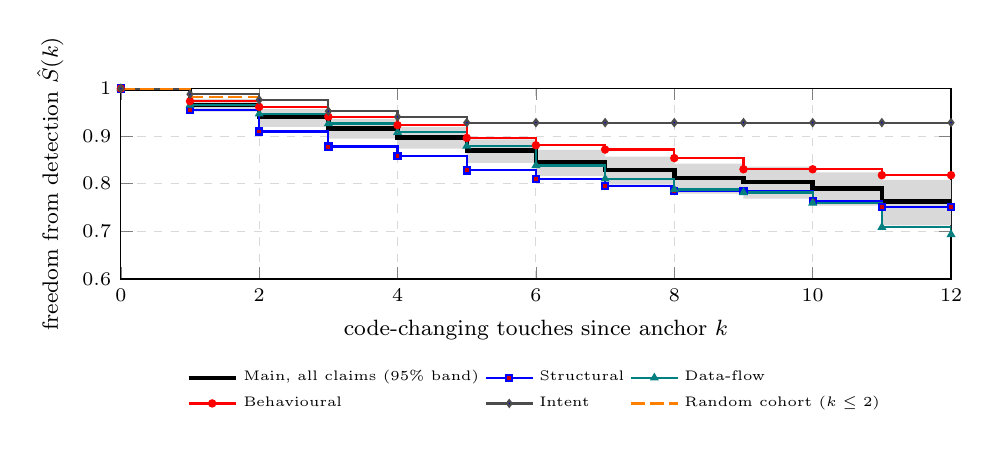
\begin{tikzpicture}
\begin{axis}[width=\columnwidth,height=4.0cm,xlabel={code-changing touches since anchor $k$},ylabel={freedom from detection $\hat S(k)$},
  xmin=0,xmax=12,ymin=0.6,ymax=1.0,xtick={0,2,...,12},grid=major,grid style={dashed,gray!30},
  legend style={at={(0.5,-0.42)},anchor=north,font=\tiny,cells={anchor=west},draw=none},legend columns=3,
  tick label style={font=\scriptsize},label style={font=\footnotesize}]
\addplot[name path=lo,const plot,draw=none,forget plot] coordinates {(0,1.0000) (1,0.9517) (2,0.9195) (3,0.8948) (4,0.8736) (5,0.8441) (6,0.8168) (7,0.7980) (8,0.7790) (9,0.7687) (10,0.7538) (11,0.7124) (12,0.7021)};
\addplot[name path=hi,const plot,draw=none,forget plot] coordinates {(0,1.0000) (1,0.9775) (2,0.9569) (3,0.9365) (4,0.9194) (5,0.8932) (6,0.8712) (7,0.8572) (8,0.8424) (9,0.8361) (10,0.8240) (11,0.8079) (12,0.8067)};
\addplot[black!15,forget plot] fill between[of=lo and hi];
\addplot+[const plot, black, mark=none, ultra thick] coordinates {(0,1.0000) (1,0.9653) (2,0.9402) (3,0.9158) (4,0.8973) (5,0.8698) (6,0.8452) (7,0.8283) (8,0.8124) (9,0.8037) (10,0.7898) (11,0.7627) (12,0.7574)};
\addlegendentry{Main, all claims (95\% band)}
\addplot+[const plot, blue,mark=square*, mark size=1.1pt, thick] coordinates {(0,1.0000) (1,0.9549) (2,0.9097) (3,0.8781) (4,0.8578) (5,0.8281) (6,0.8094) (7,0.7948) (8,0.7846) (9,0.7846) (10,0.7645) (11,0.7513) (12,0.7513)};
\addlegendentry{Structural}
\addplot+[const plot, teal,mark=triangle*, mark size=1.1pt, thick] coordinates {(0,1.0000) (1,0.9652) (2,0.9468) (3,0.9264) (4,0.9080) (5,0.8792) (6,0.8385) (7,0.8104) (8,0.7879) (9,0.7817) (10,0.7598) (11,0.7086) (12,0.6935)};
\addlegendentry{Data-flow}
\addplot+[const plot, red,mark=*, mark size=1.1pt, thick] coordinates {(0,1.0000) (1,0.9734) (2,0.9615) (3,0.9408) (4,0.9231) (5,0.8963) (6,0.8809) (7,0.8718) (8,0.8539) (9,0.8304) (10,0.8304) (11,0.8180) (12,0.8180)};
\addlegendentry{Behavioural}
\addplot+[const plot, black!70,mark=diamond*, mark size=1.1pt, thick] coordinates {(0,1.0000) (1,0.9881) (2,0.9762) (3,0.9524) (4,0.9405) (5,0.9284) (6,0.9284) (7,0.9284) (8,0.9284) (9,0.9284) (10,0.9284) (11,0.9284) (12,0.9284)};
\addlegendentry{Intent}
\addplot+[const plot, orange,dash pattern=on 5pt off 2pt,mark=none,very thick, mark size=1.1pt, thick] coordinates {(0,1.0000) (1,0.9817) (2,0.9707)};
\addlegendentry{Random cohort ($k\le2$)}
\end{axis}
\end{tikzpicture}
\caption{Kaplan--Meier freedom from judge-detected contradiction: future-active main cohort (all, cluster-bootstrap band, by type) and random cohort.}
\label{fig:km}
\end{figure}


\textbf{When detections appear.} Table~\ref{tab:survival} and Fig.~\ref{fig:km} describe the future-active, trackable main cohort. Of \XMainN{} anchor-supported claims, \XMainDeaths{} receive a contradiction over follow-up to touch \XKMax{}. At six touches, $\hat S(6)=\XMainSK$ [\XMainSKLo,\XMainSKHi]; the 10\% detection threshold is reached at touch \XMainTNineZero{}. By touch \XKMax{}, $\hat S=\XMainSKmax$, so the median detection time is not observed. These results show detections emerging after initially supported explanations have been retained; they do not establish when the underlying claims became false. By touch six, 208 detections occur in 150 function--touch groups, including 97 in 39 groups with multiple detected claims, reinforcing the need to account for shared functions.

\textbf{Activity and observation matter.} The random cohort contributes only \XRandomAtRiskOne{} claims in \XRandomFuncsAtRiskOne{} touched functions. By touch three, only \XRandomAtRiskThree{} claims in \XRandomFuncsAtRiskThree{} functions remain at risk; under our minimum of 30 claims in five functions, we report its curve only through touch \XRandomKReliable{} ($\hat S=\XRandomSKr$). Its high one-year freedom from detection (\XRandomSThreeSixFived{}, versus \XMainSThreeSixFived{} in the main cohort) therefore cannot be read as stronger claim durability: many functions receive no local edit. Counting removal/rename as an event changes the random estimate to \XRandomSThreeSixFivedRmdeath{} [\XRandomSThreeSixFivedRmdeathLo,\XRandomSThreeSixFivedRmdeathHi]. With few affected functions and selection on future activity, these contrasts do not establish a population ordering. Full calendar-time and competing-risk analyses are archived.

\textbf{Sensitivity to observation rules.} Censoring before the first unresolved verdict gives $\hat S(6)=\XUnresolvedCensorS$; counting unresolved as an event gives \XUnresolvedEventS{} (primary \XMainSK{}; \XUnresolvedClaims{} affected claims). The choice matters, although these estimates remain much closer to each other than to the Llama replay below. Unchanged-code checks yield \XPlaceboNCon{} contradictions in \XPlaceboNLooks{} looks, all in anchor retests; real unchanged versions yield 0/\XPlaceboVersionsN{}. The constant-error placebo scenario gives $\hat S(6)=\XMainSKCorrected$ [\XMainSKCorrectedLo,\XMainSKCorrectedHi]. This small change is conditional on error transfer from unchanged to changed code; the human event review demonstrates why that assumption cannot calibrate the primary curve.

\textbf{Which edits warrant attention?} Larger function edits are associated with more Qwen detections: HR \XLogLinesFnIqrHr{} [\XLogLinesFnIqrHrLo,\XLogLinesFnIqrHrHi] per inter-quartile range of lines changed. However, AUC \XHOneAucFn{} indicates only moderate discrimination over \XHOneNPairs{} analysis rows, \XHOneZeroShare\% of which have no event. Churn may help prioritize review, but these results do not establish an effective automatic refresh trigger. Claim-type contrasts are less stable: the apparent intent advantage (HR \XCloglogTyIntent{} [\XCloglogTyIntentLo,\XCloglogTyIntentHi] against data-flow) rests on \XHTwoIntentDeaths{} events, \XHTwoIntentDeathsClick{} in three click pager functions. We therefore infer no ordering by claim type.

Whole-text prompts v1/v2 flag every queried touch, including unchanged anchors; v3 barely discriminates (AUC \XHThreeVThreeAuc{} [\XHThreeVThreeAucLo,\XHThreeVThreeAucHi]). This failed prompt diagnostic leaves comparison with published JIT detectors open. The docstring contrast is also descriptive because generator exposure, claim granularity and initial eligibility differ. All coefficients and negative results remain in the artifact.

\textbf{Reliability and human audit.} Reweighted to the population strata (\XAFramePos{}/\XAFrameNeg{} touches with/without a death), the archived judges agree on \XAJudgeCommitAgreePct\% of verdicts ($\kappa=\XAJudgeCommitKappa$; $\kappa=\XAJudgeCommitKappaDead$ for contradicted vs.\ not). \XSecondModel{} confirms \XAJudgeCommitPrecision\% of bulk contradictions and contradicts \XAJudgeCommitSecondConWhereBulkNot\% of claims the bulk judge kept: this proxy disagrees in both directions and cannot calibrate $\hat S$. Separately, two self-reported blinded raters audited the same 400 records stratified by stage and bulk verdict. They agree on \XTwoRaterAgree\% ($\kappa=\XTwoRaterKappa$; weighted agreement \XTwoRaterWeightedAgree\%), with \XTwoRaterDisagreements{} disagreements resolved by a self-reported independent blinded adjudicator (Table~\ref{tab:audit}). The resulting reference labels all 134 sampled bulk-\textsc{con} records as \textsc{con}, yielding observed agreement 134/134 (exact 95\% lower limit 97.3\%) in that sampled stratum; among 297 resolved reference labels, bulk-\textsc{con} sensitivity is 134/137=97.8\%. These are not semantic PPV/recall: post-plan sampling, unresolved labels, self-reported blinding, and possible rater bias prevent that interpretation.

\begin{table}[t]
\centering\small
\caption{Two-rater audit reference of 400 recorded judgments. Rows are bulk-model labels; columns are final audit labels.}
\label{tab:audit}
\begin{tabular}{lrrr}
\toprule
 & \textsc{sup} & \textsc{con} & \textsc{unr}\\
\midrule
Bulk \textsc{sup} & 132 & 1 & 0\\
Bulk \textsc{con} & 0 & 134 & 0\\
Bulk \textsc{unr} & 28 & 2 & 103\\
\bottomrule
\end{tabular}
\end{table}

\section{Discussion and Research Agenda}\label{sec:discussion}

\textbf{Measurement changes the maintenance story.} Under Qwen, 10\% of initially supported claims receive a detection by touch four, and roughly 15\% by touch six. A full Llama replay of the same 129 functions gives $\hat S(6)=\XLlamaFullSsix$ [\XLlamaFullSsixLo,\XLlamaFullSsixHi] among \XLlamaFullN{} Llama-supported anchor claims, compared with \XMainN{} under Qwen. Anchor agreement is \XLlamaAnchorAgree\% ($\kappa=\XLlamaAnchorKappa$; 1,725 labels). The replay changes both eligibility and subsequent judgments, so it cannot isolate follow-up error alone. The gap would nevertheless materially affect a refresh schedule; choosing one from the primary curve would outrun the validation evidence.

\textbf{Human review changes the event count.} An independent rater relabeled all \XHumanEventAuditN{} unique observed Qwen-CON rows through touch six: \XHumanLabelConN{} contradicted, \XHumanLabelSupN{} supported and \XHumanLabelUnrN{} unresolved. Confirmation among resolved rows is \XHumanPpv\% [\XHumanPpvLo,\XHumanPpvHi\% Wilson]. Substitution yields $\hat S(6)=\XHumanLabelSsixLo$ when unresolved is an event or \XHumanLabelSsixHi{} when censored (function-cluster bootstrap \XHumanSsixBootLo--\XHumanSsixBootHi). It removes observed false positives but cannot recover missed contradictions, including after a rejected first event in the alive-only archive. The increase demonstrates the consequence of event verification; it does not establish a corrected semantic curve.

The two-rater audit and event review answer different questions. A1/A2 agree on \XTwoRaterAgree\% of \XTwoRaterN{} records ($\kappa=\XTwoRaterKappa$), yet the event rater confirms only \XHumanOverlapCon{} of \XHumanOverlapN{} shared Qwen-CON rows. Agreement within one frame therefore does not establish calibration across raters and frames. Independence and blinding are self-reported; no calibration session is documented. A next audit should use common guidelines and independently adjudicate both flagged and unflagged claims.

\textbf{Controlled checks have limited reach.} A synthetic suite detects \XMutationRecallPct\% of 100 known changes [\XMutationRecallLo--\XMutationRecallHi\% Wilson] with \XMutationFprPct\% false positives among 100 unchanged controls. Yet targeted review supports 75/77 Qwen-SUP/Llama-CON anchor rows and contradicts only 9/37 Qwen-CON/Llama-SUP rows. Success on controlled mutations can coexist with ambiguity in repository histories. These selected checks do not estimate population precision or recall. Likewise, churn offers a candidate review priority, but moderate discrimination and dependence on Qwen labels leave operational value open.

\textbf{What to validate next.} First, compare published JIT detectors and execution-based checks on frozen eligible inputs, reporting coverage as well as errors. Second, independently validate tracking across refactorings and renames: false matches create spurious follow-up, while failed matches may censor informatively. Third, collect representative adjudication of flagged and unflagged claims before fitting contamination-aware survival methods~\cite{bladt2026contaminated}; the present data do not identify that error mechanism. Future-conditioned selection, sparse random-cohort events, \XNRepos{} Python projects, one generator/prompt and non-local dependency changes constrain generalization. A larger, prospectively fixed cohort is needed before testing refresh policies or developer outcomes.

\section{Conclusion}\label{sec:conclusion}
Following retained claims makes their review timing measurable. Detections accumulate over successive edits, but model replay and human event review substantially change the estimated curve. Detector validation must precede maintenance policy. The released histories and analyses provide a starting point for that validation and for studies of targeted explanation refresh.

\noindent\textbf{Data availability.} Anonymous code and data: \url{https://claim-survival-artifact.dimpledshrimp2.chatgpt.site}.

\section*{AI-Use Disclosure}
LLMs (\XBulkModel{}, Llama 3.1 8B via Ollama and \XSecondModel{}) are experimental subjects and judges. An AI coding assistant implemented the artifact, audits and draft; statistics are rendered from saved outputs, and AI audits are not human evaluation.


\clearpage
\begingroup\scriptsize
\bibliographystyle{IEEEtran}
\bibliography{references}
\endgroup

\end{document}
